

Il tensore degli sforzi $\mathbb{T}$ è un tensore del secondo ordine che descrive lo stato di sforzo all'interno del mezzo continuo e permette di legare il vettore sforzo $\bm{t_n}$ agente su una superficie elementare e il versore normale $\bh{n}$ alla superficie.
Si considera in un mezzo continuo non polare\footnote{
 All'interno del mezzo continuo, le particelle adiacenti si scambiano unicamente forze elementari, non momenti.
}, e si ricava il legame tra i vettori $\bm{t_n}$, $\bh{n}$ dalle condizioni di equilibrio del tetraedro di Cauchy. Siano $\bh{x}$, $\bh{y}$ e $\bh{z}$ i versori di un sistema di riferimento cartesiano centrato nel punto del continuo considerato e $\bm{t_x}$, $\bm{t_y}$ e $\bm{t_z}$ i vettori sforzo agenti sulle facce del tetraedro di area $dS_x$, $dS_y$ e $dS_z$ con le normali orientate come i rispettivi versori della base, come rappresentato in figura \ref{fig:tetraedroCauchy}. Sia $\bm{t_n}$ il vettore sforzo agente sulla faccia ``inclinata'' di area $dS$ del tetraedro di Cauchy, con normale $\bh{n}$.

\begin{figure}[h!]
\centering
 \includegraphics[width=0.60\textwidth]{./fig/cauchy}
\caption{tetraedro di Cauchy}\label{fig:tetraedroCauchy}
\end{figure}

Il legame tra le aree delle facce del tetraedro è
\begin{equation}\label{eqn:surfaces}
 dS = - \dfrac{dS_x}{n_x} = - \dfrac{dS_y}{n_y} = - \dfrac{dS_z}{n_z} ,
\end{equation}
avendo indicato con $n_i$ le componenti cartesiane del versore normale $\bh{n}$, tutte negative per come è stato definito il tetraedro.

\paragraph{Bilancio di massa.}
Scriviamo il bilancio di massa e di quantità di moto del volume di controllo elementare $dV$ contenuto all'interno del tetraedro di Cauchy. Il bilancio di massa
\begin{equation}
 \f{d}{dt} \int_{dV} \rho + \oint_{\partial dV} \rho \bm{u} \cdot \bh{n} = 0 \ ,
\end{equation}
diventa
\begin{equation}\label{eqn:dV:mass}
\begin{aligned}
 0 = & \p{}{t}\big( \rho + O(d\ell) \big) dV
     + \big( \rho \bm{u} \cdot \bh{x} + O(d\ell) \big) dS_x
     + \big( \rho \bm{u} \cdot \bh{y} + O(d\ell) \big) dS_y \\
   & + \big( \rho \bm{u} \cdot \bh{z} + O(d\ell) \big) dS_z
     + \big( \rho \bm{u} \cdot \bh{n} + O(d\ell) \big) dS \ ,
\end{aligned}
\end{equation}
avendo scritto esplicitamente la dipendenza delle grandezze nel volume e sulle superfici da infinitesimi di ordine $O(d\ell)$, essendo $O(d\ell)$ l'ordine di grandezza delle dimensioni lineari del tetraedro di Cauchy, come ad esempio la lunghezza degli spigoli. Le superfici hanno ordine $O(dS) = O(d\ell^2)$, mentre il volume ha ordine $O(dV) = O(d\ell^3)$. Utilizzando le relazioni (\ref{eqn:surfaces}), facendo tendere $d\ell$ a zero, trascurando gli ifninitesimi di ordine superiore, i termini di ordine $O(d\ell^2)$ si riducono all'identità
\begin{equation}
 \bm{u} \cdot \bh{n} = u_x n_x + u_y n_y + u_z \ .
\end{equation}

\paragraph{Bilancio della quantità di moto.}
Il bliancio di quantità di moto per il tetraedro di Cauchy
\begin{equation}
 \f{d}{dt} \int_V \rho \bm{u} + \oint_{\partial dV} \rho \bm{u} \bm{u} \cdot \bh{n} = \int_{dV} \rho \bm{g} + \oint_{\partial dV} \bm{t_n} \ ,
\end{equation}
diventa
\begin{equation}
\begin{aligned}
 & \p{}{t} \big( \rho \bm{u} + O(d\ell) \big)dV +
 \sum_{i \in \{x,y,z\}} \big( \rho \bm{u} \bm{u} \cdot \bh{x}_i + O(d\ell) \big)dS_i +
                \big( \rho \bm{u} \bm{u} \cdot \bh{n}   + O(d\ell) \big)dS   = \\
 & = \big( \rho \bm{g} + o(d\ell) \big) dV +
     \big( \bm{t_x} + O(d\ell) \big) dS_x +
     \big( \bm{t_y} + O(d\ell) \big) dS_y + \\
 & \hspace{4.5cm} + \big( \bm{t_z} + O(d\ell) \big) dS_z +
     \big( \bm{t_n} + O(d\ell) \big) dS \ .
\end{aligned}
\end{equation}
I termini ``più grandi'' sono infinitesimi di ordine $O(d\ell^2)$.
Utilizzando il bilancio di massa, non è difficile verificare che i termini di flusso di quantità di moto danno un contributo nullo di ordine $O(d\ell^2)$. I termini di volume sono infinitesimi di ordine $O(d\ell^3)$.
Facendo tendere $d\ell$ a zero e trascurando tutti gli infinitesimi di ordine superiore a $O(d\ell)$ si ottiene
\begin{equation}\label{eqn:dV:equil}
\begin{aligned}
 \bm{0} & = \bm{t_n} dS + \bm{t_x} dS_x + \bm{t_y} dS_y + \bm{t_z} dS_z = \\
  & = ( \bm{t_n} - \bm{t_x} n_x - \bm{t_y} n_y - \bm{t_z} n_z ) dS  \qquad \rightarrow \qquad \bm{t_n} = \bm{t_x} n_x + \bm{t_y} n_y + \bm{t_z} n_z \ .
\end{aligned}
\end{equation}
Se si esprimono i vettori utilizzando la base $\{\bh{x}, \, \bh{y}, \, \bh{z} \}$,
\begin{equation}\label{eqn:t:comp}
  \bm{t_i} = t_{ix} \bh{x} + t_{iy} \bh{y} + t_{iz} \bh{z} \ ,
\end{equation}
si può scrivere la relazione (\ref{eqn:dV:equil}) per trovare la relazione tra il versore $\bh{n}$ e il vettore sforzo $\bm{t_n}$
\begin{equation}
\begin{aligned}
  \bm{t_n} & = \bm{t_x} n_x + \bm{t_y} n_y + \bm{t_z} n_z \\ 
 & = n_x ( t_{xx} \bm{\hat{x}} + t_{xy} \bm{\hat{y}} +  t_{xz} \bm{\hat{z}} ) % + \\
   + n_y ( t_{yx} \bm{\hat{x}} + t_{yy} \bm{\hat{y}} +  t_{yz} \bm{\hat{z}} ) % + \\
   + n_z ( t_{zx} \bm{\hat{x}} + t_{zy} \bm{\hat{y}} +  t_{zz} \bm{\hat{z}} ) = \\
 & = ( \bh{n} \cdot \bh{x} ) ( t_{xx} \bm{\hat{x}} + t_{xy} \bm{\hat{y}} +  t_{xz} \bm{\hat{z}} )% + \\
   + ( \bh{n} \cdot \bh{y} ) ( t_{yx} \bm{\hat{x}} + t_{yy} \bm{\hat{y}} +  t_{yz} \bm{\hat{z}} )% + \\
   + ( \bh{n} \cdot \bh{z} ) ( t_{zx} \bm{\hat{x}} + t_{zy} \bm{\hat{y}} +  t_{zz} \bm{\hat{z}} ) = \\
%   & = ( \bm{n} \cdot \bm{\hat{x}} ) \bm{t_x} + 
%       ( \bm{n} \cdot \bm{\hat{y}} ) \bm{t_y} + 
%       ( \bm{n} \cdot \bm{\hat{z}} ) \bm{t_z} = \\
    & = \bh{n} \cdot ( t_{xx} \bm{\hat{x}} \otimes \bm{\hat{x}} + 
                       t_{xy} \bm{\hat{x}} \otimes \bm{\hat{y}} +
                       t_{xz} \bm{\hat{x}} \otimes \bm{\hat{z}} + \\
            & \qquad + t_{yx} \bm{\hat{y}} \otimes \bm{\hat{x}} + 
                       t_{yy} \bm{\hat{y}} \otimes \bm{\hat{y}} +
                       t_{yz} \bm{\hat{y}} \otimes \bm{\hat{z}} + \\
            & \qquad + t_{zx} \bm{\hat{z}} \otimes \bm{\hat{x}} + 
                       t_{zy} \bm{\hat{z}} \otimes \bm{\hat{y}} +
                       t_{zz} \bm{\hat{z}} \otimes \bm{\hat{z}} ) =
     \bm{\hat{n}} \cdot \mathbb{T}  \ ,
\end{aligned}  
\end{equation}
avendo utilizzato l'identità $(\bm{a} \cdot \bm{b})\bm{c} = \bm{a} \cdot (\bm{b}\otimes\bm{c})$, per isolare il versore $\bh{n}$ dal tensore degli sforzi $\mathbb{T}$. Avendo utilizzato la definizione (\ref{eqn:t:comp}) delle componenti cartesiane dei vettori dello sforzo agente sulle facce del tetraedro di Cauchy, il primo indice delle componenti del tensore degli sforzi indica la faccia sulla quale agisce lo sforzo, il secondo indice la sua componente cartesiana, cosicché la componente $t_{ij}$ indica la componente cartesiana $j$-esima agente sulla $i$-esima faccia del tetraedro di Cauchy.
%
\newline \noindent
\textbf{Osservazione 1.} Utilizzando le convenzioni scelte in precedenza, il vettore sforzo si ottiene con la relazione
\begin{equation}
 \bm{t_n} = \bh{n} \cdot \mathbb{T} \qquad , \qquad t_{n,i} = n_j t_{ji} \ ,
\end{equation}
che in generale differisce dall'operazione $\mathbb{T} \cdot \bh{n}$, la cui $i$-esima componente cartesiana è $n_j t_{ij}$.
%
\newline \noindent
\textbf{Osservazione 2.} Se il tensore $\mathbb{S}$ è simmetrico (e quindi le sue componenti con indici misti sono uguali, $S_{ij} = S_{ji}$), la moltiplicazione a sinista o a destra di un vettore tramite il prodotto ``punto'' dà lo stesso risultato,
\begin{equation}
 \bm{a} \cdot \mathbb{S} = \mathbb{S} \cdot \bm{a} \qquad , \qquad 
 a_j S_{ji} = S_{ij} a_j \ .
\end{equation}
%
\newline \noindent
\textbf{Osservazione 3.} Il tensore degli sforzi per mezzi continui non polari è simmetrico. Questo permette di ottenere la corretta relazione tra versore normale alla superficie e vettore sforzo, anche in seguito ad alcune imprecisioni nell'utilizzo delle operazioni tensoriali, come uno scambio di indici nel tensore degli sforzi.
%
\newline \noindent
\textbf{Osservazione 4.} Non è stata prestata mai attenzione alla posizione degli indici poiché si è lavorato sempre con basi ortonormali, come la base cartesiana.
%
\newline \noindent
\textbf{Osservazione 5.} \'E possibile utilizzare altre convenzioni nella definizione delle componenti dei vettori sforzo agenti sulle facce del tetraedro di Cauchy, che portano a una diversa interpretazione degli indici e alla rappresentazione della relazione di Cauchy.

\paragraph{Bilancio della quantità di moto.} Dal bilancio del momento della quantità di moto in forma differenziale, è possibile ricavare la condizione di simmetria del tensore degli sforzi. Per ricavare il bilancio in forma differenziale, si parte dal bilancio integrale del momento della quantità di moto per un volume di controllo $V$ fisso nello spazio,
\begin{equation}
 \f{d}{dt} \int_V \rho \bm{r} \times \bm{u} + \oint_{\partial V} \rho \bm{r} \times \bm{u} \bm{u} \cdot \bh{n} = \int_{V} \rho \bm{r} \times \bm{g} + \oint_{\partial V} \bm{r} \times \bm{t_n} \ ,
\end{equation}
dove $\bm{r}$ è il raggio vettore tra il punto del fluido e il polo, qui fisso nello spazio, rispetto al quale è definito il momento della quantità di moto. Si trasformano i due termini di superficie in integrali di volume. Il termine di flusso diventa,
\begin{equation}
\begin{aligned}
  \oint_{\partial V} \rho \bm{r} \times \bm{u} \bm{u} \cdot \bh{n} & =
  \oint_{\partial V} \rho \epsilon_{ijk} r_j u_k u_l n_l = \\
 & = \int_{V} \partial_l \left( \rho \epsilon_{ijk} r_j u_k u_l \right) =
     \int_{V} \bm{\nabla} \cdot \left( \rho \bm{u} \,\,  \bm{r} \times \bm{u} \right) \ ,
\end{aligned}
\end{equation}
mentre il termine degli sforzi di superficie diventa,
\begin{equation}
\begin{aligned}
  \oint_{\partial V} \bm{r} \times \bm{t_n} = \oint_{\partial V} \bm{r} \times \left( \bm{\hat{n}} \cdot \mathbb{T} \right) & = \oint_{\partial V} \epsilon_{ijk} r_j n_l T_{lk} \\
   & = \int_{V} \partial_l \left( \epsilon_{ijk} r_j T_{lk} \right) \ .
\end{aligned}
\end{equation}
Dopo aver trasformato gli integrali di superfici in integrali di volume, sotto l'ipotesi che i campi siano sufficientemente regolari, si ricava il bilancio in forma differenziale sfruttando l'arbitrarietà del volume $V$,
\begin{equation}
 \p{}{t} \left( \rho \bm{r} \times \bm{u} \right) + \bm{\nabla} \cdot \left( \rho \bm{u} \,\,  \bm{r} \times \bm{u} \right) = \rho \bm{r} \times \bm{g} + \partial_l \left( \epsilon_{ijk} r_j T_{lk} \right) \ ,
\end{equation}
avendo utilizzato una ``notazione mista'', per esprimere nella maniera meno ambigua possibile la componente $i$-esima del termine degli sforzi.

\noindent
Si usa ora la formula per la derivata del prodotto di funzioni per manipolare il secondo termine dell'equazione,
\begin{equation}
\begin{aligned}
  \bm{\nabla} \cdot \left( \rho \bm{u} \,\,  \bm{r} \times \bm{u} \right) & =
  \partial_l \left( \rho u_l \epsilon_{ijk} r_j u_k \right) \\
  & = \epsilon_{ijk} r_j \partial_l \left( \rho u_l u_k \right) +
      \underbrace{\epsilon_{ijk} \partial_l r_j}_{\epsilon_{ijk} \delta_{lj}} \left( \rho u_l u_k \right) \\
  & = \epsilon_{ijk} r_j \partial_l \left( \rho u_l u_k \right) +
      \underbrace{\epsilon_{ilk} \left( \rho u_l u_k \right)}_{ = 0 } 
  = \bm{r} \times \left( \rho \bm{u} \bm{u} \right)
\end{aligned}
\end{equation}
dove è nullo il termine $\epsilon_{ilk} \left(rho u_l u_k \right)$, poiché il contenuto della parentesi è un tensore del secondo ordine simmetrico. Si usa ancora la formula per la derivata del prodotto di funzioni per manipolare l'ultimo termine,
\begin{equation}
 \partial_l( \epsilon_{ijk} r_j T_{lk} ) = \epsilon_{ijk} r_j \partial_l T_{lk} + 
  \epsilon_{ijk} T_{jk} \ ,
\end{equation}
e poter scrivere il bilancio della quantità di moto in forma differenziale come
\begin{equation}
 \bm{r} \times \left[ \p{}{t} \left( \rho \bm{u} \right) + \bm{\nabla} \cdot \left( \rho \bm{u} \bm{u} \right) - \rho \bm{g} - \bm{\nabla} \cdot \mathbb{T} \right] = \epsilon_{ijk} T_{jk} \ .
\end{equation}
Il contenuto della parentesi quadra è identicamente nullo, poiché coincide con il bilancio della quantità di moto. Questo implica che,
\begin{equation}
  \epsilon_{ijk} T_{jk} = 0 \ ,
\end{equation}
e che quindi $T_{jk} = T_{kj}$, cioè che il tensore degli sforzi sia simmetrico.


